\documentclass[
  final,
  babelLanguage=italian,
  %desktopVersion,
  %showtrims,
  %overleaf,
]{anecdote}

%\graphicspath{{./assets/photos/300dpi/}}
\graphicspath{{./assets/photos/92dpi/}}

% Page size: 6x9 inch
% Body text: 10.5 / 15 pt

\usepackage{local}

%% Details of the book
%% ===================

\title{Ajahn Chah Insegnamenti}
\subtitle{}
\author{Ajahn Chah}
\publisher{The Publisher}
\date{2018-10-18}
\editionInfo{\textit{First edition}, printed in TODO Country, 2017}% TODO update edition info
\ISBN{000-000-0000-00-0}% TODO update ISBN

% === Metadata ===

\hypersetup{
  pdftitle={\thetitle},
  pdfauthor={\theauthor},
  pdfcopyright={Copyright (C) 2017, \thePublisher},
  pdfsubject={},% TODO subject
  pdfkeywords={},% TODO keywords
  pdflicenseurl={https://creativecommons.org/licenses/by-nc-nd/4.0/},
  pdfcontacturl={},
  pdflang={it},
}

\pdfinfo{%
  /Title (\thetitle)%
  /Author (\theauthor)
  /Subject (subject)% TODO subject
  /Keywords (keywords)% TODO keywords
  /GTS_PDFXVersion (PDF/X-1:2001)%
  /GTS_PDFXConformance (PDF/X-1a:2001)%
}

%% === Load further packages ===

%% === Hyphenation exceptions and corrections ===

\hyphenation{London}

\begin{document}

\frontmatter

\ifdesktopversion
\desktopCover{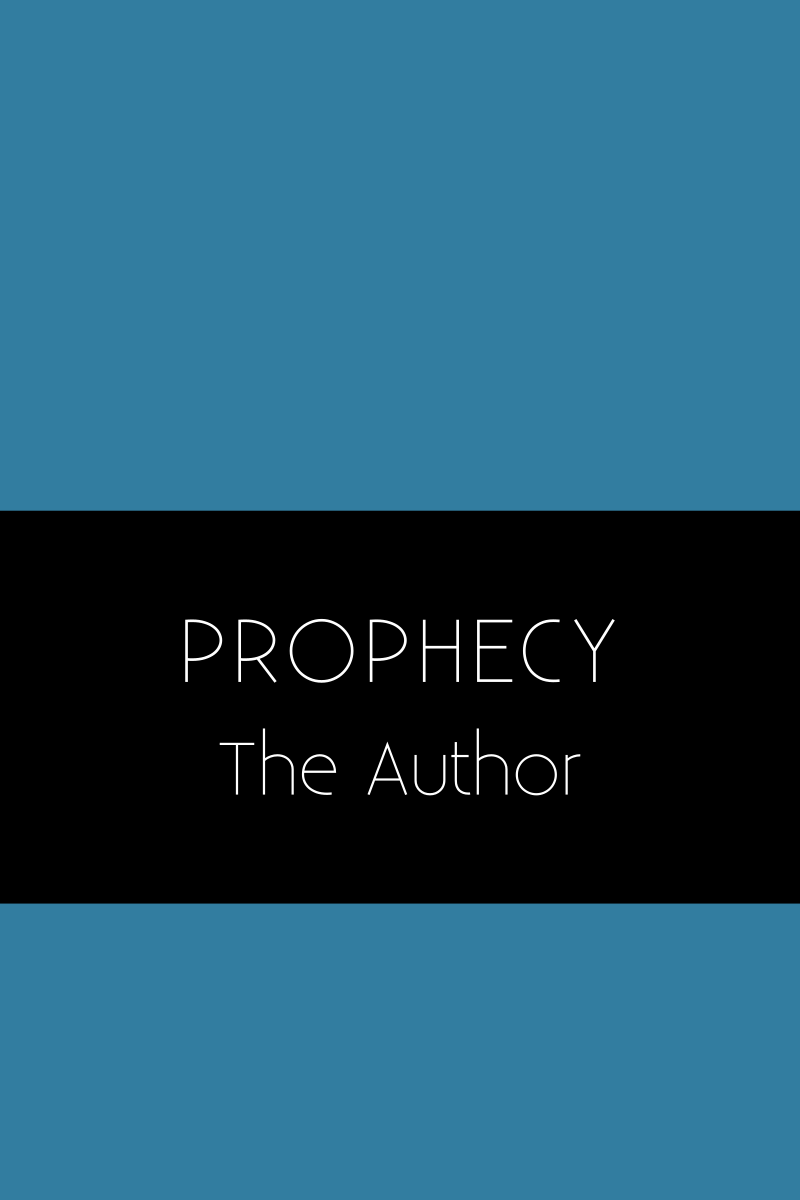
\includegraphics[height=\paperheight]{./desktop-cover.png}}
\fi

\cleartorecto
\thispagestyle{empty}
\vspace*{5em}

{\centering

\settowidth{\titleLength}{%
  {\fontsize{16}{16}\selectfont\ebGaramondSmallCapsFont\textls{Insegnamenti}}%
}

{\fontsize{16}{16}\selectfont\ebGaramondSmallCapsFont\textls{Insegnamenti}}\\[0.3\baselineskip]
\setlength{\xheight}{\heightof{X}}
\raisebox{0.5\xheight}{\color[gray]{0.4}\rule{\titleLength}{0.25pt}}\\[0.3\baselineskip]
{\itshape
\thesubtitle}

\vfill

\theauthor

\vspace*{5em}

}



\cleartoverso
\thispagestyle{empty}

{\copyrightsize
\centering
\setlength{\parindent}{0pt}%
\setlength{\parskip}{0.8\baselineskip}%

\thetitle\ -- \thesubtitle\\
by \theauthor

Published by \thePublisher

ISBN \theISBN

Copyright \copyright\ \thePublisher\ 2017

Cover Photograph: The Person

\vfill

{\footnotesize

This work is licensed under a Creative Commons\\
Attribution-NonCommercial-NoDerivatives 4.0 International~License.

Produced with the \LaTeX\ typesetting system, set in Gentium and Crimson Roman.

\theEditionInfo

}}


\cleartorecto
\thispagestyle{empty}

\mbox{}
\vfill

\begin{quote}
\centering

Per l’aiuto ricevuto nella preparazione di questo libro\\
vogliamo esprimere la nostra gratitudine a molte persone,\\
in particolare al gruppo Kataññutā della Malesia, Singapore e Australia\\
che ne ha reso possibile la stampa.

\end{quote}

\vspace*{4\baselineskip}

\vfill
\mbox{}



\cleartorecto
\tableofcontents*

\chapter{Foreword}

Nullam eu ante vel est convallis dignissim. Fusce suscipit, wisi nec facilisis
facilisis, est dui fermentum leo, quis tempor ligula erat quis odio. Nunc porta
vulputate tellus. Nunc rutrum turpis sed pede. Sed bibendum. Aliquam posuere.
Nunc aliquet, augue nec adipiscing interdum, lacus tellus malesuada massa, quis
varius mi purus non odio. Pellentesque condimentum, magna ut suscipit hendrerit,
ipsum augue ornare nulla, non luctus diam neque sit amet urna. Curabitur
vulputate vestibulum lorem. Fusce sagittis, libero non molestie mollis, magna
orci ultrices dolor, at vulputate neque nulla lacinia eros. Sed id ligula quis
est convallis tempor. Curabitur lacinia pulvinar nibh. Nam a sapien.

\bigskip

{\raggedleft
  Reviewer Person\\
  July 2017
\par}


\chapter{Prefazione}

Gli insegnamenti del venerabile Ajahn Chah tradotti e resi fruibili in
questa edizione sono diretti e chiari. Mi dà molta gioia sapere che una
tale saggezza stia per essere ampiamente diffusa.

Ho avuto la grande fortuna di vivere con Ajahn Chah o di stargli vicino
tra il 1967 e il 1977, gli anni centrali del suo insegnamento. Dopo aver
ricevuto l'ordinazione nel maggio del 1967 nella Thailandia del
nord-est, nella provincia di Nong Khai, il mio precettore mi inviò al
Wat Nong Pah Pong per la formazione. Fu durante il mio primo ritiro
delle piogge (\emph{vassa}) in quel monastero, mentre vivevo sotto la
guida di Ajahn Chah, che davvero crebbero la mia fede e la mia fiducia
nei riguardi di questo modo di praticare. Durante quei dieci anni ho
avuto l'opportunità di studiare e di comprendere la relazione tra il
Dhamma e il Vinaya (la disciplina monastica), di sviluppare una visione
profonda della vacuità e della forma, e di riconoscere la sofferenza
causata dall'ignoranza dei miei attaccamenti ai fenomeni condizionati.

L'approccio di Ajahn Chah all'insegnamento e alla formazione è semplice
e pratico. È uno strumento perfetto per rendere chiare le illusioni del
sé, le presunzioni culturali e sociali nonché i processi del nostro
pensiero. Ora i suoi insegnamenti, originariamente registrati, sono
tradotti, disponibili e facilmente raggiungibili. Sono perciò grato sia
a chi ha lavorato alla traduzione e alla compilazione sia agli sponsor
che hanno reso possibile la distribuzione gratuita.

L'insegnamento del Buddha è un grande dono, ancor più necessario oggi
per far fronte ai problemi delle società contemporanee. Che questa
raccolta di insegnamenti possa essere di beneficio a molte persone.

\bigskip

{\raggedleft
  Luang Por Sumedho,\\
  novembre 2010
\par}

\clearpage

Gli insegnamenti di Ajahn Chah erano disarmanti per la loro immediatezza
e stimolanti per la loro rilevanza. Egli avrebbe detto: «~Se lasciate
andare un po', avrete un po' di pace. Se lasciate andare molto, avrete
molta pace. E se lasciate andare del tutto, avrete una pace totale.~»

Stare vicino a lui significava essere vicino al miglior amico possibile.
Quando eravamo maldestri o sbagliavamo non rideva di noi, rideva con
noi. Quando stavamo soffrendo per i dubbi, non ci rimproverava per
mancanza di fede, ma ci parlava dei tempi in cui lui stesso aveva
dubitato così tanto da pensare che la sua testa sarebbe scoppiata. E se
voleva ispirarci diligenza nella pratica, si sedeva in meditazione con
noi, recitava i canti con noi e lavorava con noi. Il nostro inciampare e
annaspare non erano mai giudicati, ma considerati in un modo che dava
dignità ai nostri sforzi, non disperazione. Gli incoraggiamenti di Ajahn
Chah a lasciar andare non erano né una tecnica né un toccasana; si
trattava piuttosto di condividere la luce che aveva trovato nella sua
pratica, per far sì che anche noi potessimo trovare la direzione verso
la libertà dalla sofferenza.

Osservando la mole di questa edizione, i lettori potrebbero
meravigliarsi del fatto che, sebbene gli insegnamenti fossero stati così
semplici, siano state necessarie così tante parole per esprimerli.
Questo è dovuto al fatto che siamo in grado di generare confusione in
numerosissimi modi. Ajahn Chah conosceva il luogo della pace perfetta ed
era contento di dimorarvi. Egli, però, era anche instancabile nei suoi
sforzi di guidare gli altri. Vivendo con lui, a volte pareva che ci
fosse indicato quel luogo di benessere, un invito a godere i frutti
della pratica. Più spesso era come se lui stesse percorrendo la strada
al nostro fianco.

Come vedrete, questi insegnamenti non sono un manuale di buddhismo. Qui
non troverete neanche le soluzioni a tutti i vostri problemi. Gli
insegnamenti di Ajahn Chah mirano a metterci in contatto con le nostre
domande più profonde e ad aiutarci ad ascoltarle, pazientemente e
gentilmente, fino a quando non si rivela la via da seguire.

I discorsi presenti in questa raccolta sono stati registrati, trascritti
e tradotti molti anni fa e sono in un certo qual modo lontani dalla loro
fonte. Ovviamente, se letti con un cuore ricettivo e con una mente
raccolta, queste ``indicazioni'' verso la Verità forniranno ispirazione
e istruzioni preziose. L'umiltà, la gioia e la saggezza di Ajahn Chah
risplendono nelle sue parole, illuminando il Sentiero mentre lo
percorriamo. Sono trascorsi quasi vent'anni da quando Ajahn Chah è
morto. Grazie al supporto di sponsor generosi, abbiamo colto questa
opportunità di mettere insieme tutti i discorsi disponibili per
distribuzione gratuita e di presentarli in una forma che speriamo possa
essere facilmente accessibile a tutti coloro che si sentono attratti
dalla pace.

\bigskip

{\raggedleft
  Ajahn Munindo,\\
  aprile 2011
\par}


% Page 1 is the first page of the first chapter.
\mainmatter

\chapterNote{Chapter one subtitle}

\chapter{Chapter One Title}
\tocChapterNote{Chapter one subtitle}

Aliquam erat volutpat. Nunc eleifend leo vitae magna. In id erat non orci
commodo lobortis. Proin neque massa, cursus ut, gravida ut, lobortis eget,
lacus. Sed diam. Praesent fermentum tempor tellus. Nullam tempus. Mauris ac
felis vel velit tristique imperdiet. Donec at pede. Etiam vel neque nec dui
dignissim bibendum. Vivamus id enim. Phasellus neque orci, porta a, aliquet
quis, semper a, massa. Phasellus purus. Pellentesque tristique imperdiet tortor.
Nam euismod tellus id erat.


\chapterNote{Chapter two subtitle}

\chapter{Chapter Two Title}
\tocChapterNote{Chapter two subtitle}

Nullam eu ante vel est convallis dignissim. Fusce suscipit, wisi nec facilisis
facilisis, est dui fermentum leo, quis tempor ligula erat quis odio. Nunc porta
vulputate tellus. Nunc rutrum turpis sed pede. Sed bibendum. Aliquam posuere.
Nunc aliquet, augue nec adipiscing interdum, lacus tellus malesuada massa, quis
varius mi purus non odio. Pellentesque condimentum, magna ut suscipit hendrerit,
ipsum augue ornare nulla, non luctus diam neque sit amet urna. Curabitur
vulputate vestibulum lorem. Fusce sagittis, libero non molestie mollis, magna
orci ultrices dolor, at vulputate neque nulla lacinia eros. Sed id ligula quis
est convallis tempor. Curabitur lacinia pulvinar nibh. Nam a sapien.




\backmatter

\chapterFootnote{%
  Si è cercato quanto più possibile di rispettare la forma corretta sia dal
  punto di vista grammaticale che tecnico di termini e concetti in italiano; i
  sostantivi in lingua pāli sono in genere allo stato tematico, mentre la forma
  nominativa, singolare o plurale, è indicata tra parentesi tonde qualora essa
  corrisponda a quella di solito ricorrente. Per alcune integrazioni ci si è
  avvalsi del glossario contenuto in \emph{La Rivelazione del Buddha}, I:
  \emph{I~testi antichi}, a cura di R. Gnoli, Milano 2007 (I Meridiani. Classici
  dello Spirito).%
}

\chapter{Glossario}

\begin{glossarydescription}

% === A ===

\item[Abhidhamma.] (1) Nei discorsi del Canone in pāli questo termine
  indica semplicemente il ``Dhamma più elevato'', nonché un tentativo
  sistematico di definire gli insegnamenti del Buddha e di comprendere le loro
  correlazioni. (2) Terza parte del Canone in pāli, composta di trattati
  analitici basati su elenchi di categorie estratte dai discorsi del Buddha.

\item[ācariya.] Insegnante, mentore, maestro; →~\emph{ajahn};
  →~\emph{kalyāṇamitta}.

\item[adhiṭṭhāna.] Determinazione, decisione, risolutezza, impegno o
  intento che rivolge la mente in una certa direzione. È una delle dieci
  perfezioni; →~\emph{pāramī}.

\item[ajahn.] (thai: \thai{อาจารย์}) Il termine deriva da \emph{ācariya}, in pāli,
  letteralmente ``insegnante''; spesso viene utilizzato per un monaco o per una
  monaca con più di dieci anni di vita monastica.

\item[ājīvaka.] Una scuola di contemplativi contemporanea del Buddha, i
  cui seguaci ritenevano che la volontà degli esseri non fosse in grado di
  indirizzare le loro azioni e che l'universo fosse guidato dalla sorte.

\item[akusala.] Non salutare, nocivo, maldestro, non meritorio;
  →~\emph{kusala}.

\item[Ālāra Kālāma.] Il maestro che insegnò al \emph{bodhisatta} la meditazione
  nella sfera del ``senza forma'' sulla ``base del nulla'' quale più alta
  fruizione della vita santa.

\item[anāgāmin, anāgāmī.] ``Chi è senza ritorno'', ossia chi ha divelto
  tutte e cinque le catene inferiori (→~\emph{saṃyojana}) che legano la mente al
  ciclo della rinascita, e che dopo la morte apparirà in uno dei mondi di
  Brahmā, per poi entrare nel →~Nibbāna, senza mai tornare in questo
  mondo.

\item[anāgārika.] (thai: \emph{pah-kao}, \thai{ผ้าขาว}, \thai{ปะขาว})
  Letteralmente, ``non cittadino'', ossia ``senza casa''. Un postulante che ha
  assunto gli Otto →~Precetti e spesso vive con i →~\emph{bhikkhu}, oltre a
  sostenere la sua pratica di meditazione, li aiuta in alcuni lavori che il
  Vinaya impedisce loro di svolgere.

\item[ānāpānasati.] Letteralmente, ``consapevolezza dell'inspirazione e
  dell'espirazione'' o consapevolezza del respiro. Questa pratica di meditazione
  consiste nel mantenere l'attenzione e la consapevolezza sulle sensazioni del
  respiro.

\item[anatta, anattā.] Non-sé, non sostanziale, impersonale;
  →~\emph{tilakkhaṇa}.

\item[anicca, aniccā.] Incostante, instabile, impermanente;
  →~\emph{tilakkhaṇa}.

\item[añjali.] È un gesto di rispetto consistente nel congiungere le mani
  al petto al cospetto di qualcuno; oggigiorno è ancora diffuso nei paesi
  buddhisti e in India.

\item[antara-vāsaka.] →~veste monastica.

\item[ānupubbi-kathā.] Istruzione graduale. Il metodo d'insegnamento del
  Dhamma da parte del Buddha che conduce progressivamente i suoi ascoltatori per
  mezzo di argomenti via via più avanzati: la generosità (→~\emph{dāna}), la
  virtù o moralità (→~\emph{sīla}), i paradisi, gli svantaggi dei piaceri
  sensoriali, la rinuncia (→~\emph{nekkhamma}) e le Quattro Nobili Verità
  (→~\emph{ariya-sacca}).

\item[anusaya.] Predisposizione; tendenza latente. Ci sono sette tendenze
  maggiori latenti, verso le quali la mente torna in continuazione: verso la
  passione sensoriale (\emph{kāma}-\emph{rāganusaya}), l'avversione
  (\emph{patighānusaya}), le visioni errate (\emph{dhiṭṭhānusaya}), il dubbio
  (\emph{vicikicchānusaya}), l'orgoglio (\emph{mānusaya}), la passione per il
  divenire (\emph{bhava}-\emph{rāganusaya}), l'ignoranza (\emph{avijjānusaya});
  →~\emph{saṃyojana}.

\item[arahant.] Letteralmente, un ``Meritevole''; una
  persona la cui mente è libera dalle contaminazioni (→~\emph{kilesa}), che ha
  abbandonato tutte e dieci le catene (→~\emph{saṃyojana}), sia le cinque
  inferiori sia le cinque superiori che legano la mente al ciclo della
  rinascita, il cui cuore è libero dagli influssi impuri (→~\emph{āsava}), e che
  perciò non è destinato a un'altra rinascita. È anche un titolo del Buddha e il
  livello più alto dei suoi Nobili Discepoli.

\item[ārammaṇa.] Oggetto mentale, oggetto di riferimento di un metodo
  meditativo.

\item[ariya.] Nobile; chi ha ottenuto la visione trascendente in uno dei
  quattro livelli dell'Illuminazione, il più alto dei quali è quello
  dell'→~\emph{arahant}; i tre precedenti stadi sono: →~\emph{sotāpanna};
  →~\emph{sakadāgāmin}; →~\emph{anāgāmin}. Tutti insieme costoro formano la
  categoria delle Nobili Persone; →~\emph{ariya-puggala}.

\item[ariya-puggala.] Letteralmente, ``Nobile Persona''; chi ha percorso
  almeno il primo sentiero inferiore dei quattro Nobili Sentieri
  (→~\emph{magga}) o conseguito il Frutto (→~\emph{phala}) di essi. Si paragoni
  quanto detto in relazione a →~\emph{puthujjana}.

\item[ariya-sacca, ariya-saccāni.] Nobile Verità. Le Quattro Nobili Verità
  costituiscono il primo e centrale insegnamento del Buddha riguardo alla
  sofferenza, alla sua origine, alla sua cessazione e al Sentiero che conduce a
  tale cessazione (\emph{dukkha-nirodha-gāminī-paṭipadā}). La completa
  comprensione della Quattro Nobili Verità equivale alla fruizione del
  Nibbāna.

\item[asaṅkhata-dhamma.] Si veda il suo opposto →~\emph{saṅkhata-dhamma}.

\item[āsava.] Influsso impuro, macchia, fermentazione o effluenza. Le
  quattro qualità che macchiano la mente: brama sensoriale, visioni errate,
  divenire e ignoranza.

\item[asekha.] Una persona (\emph{puggala}) oltre l'addestramento, ossia
  un →~\emph{arahant}.

\item[asubha.] Non bello, da intendersi come repulsivo, ripugnante e
  sporco. Il Buddha raccomandò la contemplazione di questi aspetti del corpo
  come antidoto alla lussuria.

\item[atta, attā.] Io o sé, sostanziale, personale; a volte con
  il senso di anima; si veda il suo opposto (→~\emph{anatta}).

\item[avijjā.] Non conoscenza, ignoranza; consapevolezza offuscata;
  confusione (→~\emph{moha}) sulla natura della mente. La principale radice del
  male e della continua rinascita.

\item[āyatana.] Le basi sensoriali. Le basi interne sono gli organi dei
  sensi: occhi, orecchi, naso, lingua, corpo e mente. Le basi esterne sono i
  loro rispettivi oggetti.

% === B ===

\item[bala.] Forza, potere. Si riferisce a cinque facoltà: fede/fiducia
  (→~\emph{saddhā}), energia (→~\emph{viriya}), consapevolezza (→~\emph{sati}),
  concentrazione (→~\emph{samādhi}), saggezza (→~\emph{paññā}); queste facoltà
  vengono coltivate per spezzare le cinque catene secondarie
  (→~\emph{saṃyojana}).

\item[bhante.] Epiteto, ``venerabile signore''; viene spesso utilizzato
  quando ci si rivolge a un monaco buddhista.

\item[bhava.] Esistenza; divenire; una ``vita''. Stati dell'esistenza che
  si sviluppano nella mente e possono essere sperimentati come mondi interiori
  e/o come mondi a livello esterno. Tre sono i livelli del divenire: il livello
  dei sensi, il livello della forma e il livello dell'assenza di forma.

\item[bhāvanā.] Meditazione, sviluppo o coltivazione. Termine spesso
  utilizzato per far riferimento a \emph{citta-bhāvanā}, allo sviluppo della
  mente, o a \emph{paññā-bhāvanā}, sviluppo della saggezza;
  →~\emph{kammaṭṭhāna}.

\item[bhava-taṇhā.] Bramosia di divenire, di essere.

\item[bhikkhu.] Un monaco buddhista; un uomo che ha rinunciato al suo
  ruolo in famiglia per vivere a un livello più alto di virtù (→~\emph{sīla}) in
  accordo con il →~Vinaya in generale, e con le regole del →~\emph{Pāṭimokkha};
  →~\emph{parisā}; →~Saṅgha; →~\emph{upasampadā}.

\item[bhikkhunī.] Una monaca buddhista; una donna che ha rinunciato al suo
  ruolo in famiglia per vivere a un livello più alto di virtù (→~\emph{sīla}) in
  accordo con il →~Vinaya in generale, e con le regole del →~\emph{Pāṭimokkha};
  →~\emph{parisā}; →~Saṅgha; →~\emph{upasampadā}.

\item[bhikkhu-saṅgha.] La comunità dei monaci buddhisti; →~Saṅgha.

\item[bodhi.] Risveglio; →~Illuminazione.

\item[bodhi-pakkhiya-dhamma.] Le parti del Risveglio, ossia i trentasette
  fattori che contribuiscono al Risveglio: (1) i quattro fondamenti della
  consapevolezza (→~\emph{satipaṭṭhāna}); (2) i quattro tipi di retto sforzo
  (→~\emph{sammappadhāna}); (3) le quattro basi del potere psichico
  (→~\emph{iddhipāda}); (4) le cinque facoltà spirituali (→~\emph{indriya}); (5)
  i cinque poteri (→~\emph{bala}); (6) i sette fattori del Risveglio
  (→~\emph{bojjhaṅga}); (7) il →~Nobile Ottuplice Sentiero (\emph{magga});
  →~\emph{magga}.

\item[bodhisatta.] (sanscrito: \emph{bodhisattva}) Un essere che si impegna per
  raggiungere il Risveglio; è il termine utilizzato per descrivere il Buddha
  prima dell'Illuminazione, dall'iniziale aspirazione alla Buddhità fino al
  pieno Risveglio.

\item[bojjhaṅga.]\label{glossary-bojjhanga} I sette fattori del Risveglio: consapevolezza
  (→~\emph{sati}); investigazione dei \emph{dhamma} o stati mentali
  (→~\emph{dhamma-vicaya}); energia (→~\emph{viriya}): gioia (→~\emph{pīti});
  tranquillità (\emph{passaddhi}); concentrazione o raccoglimento
  (→~\emph{samādhi}); equanimità (→~\emph{upekkhā}).

\item[brahmacariyā.] Letteralmente, comportamento di Brahmā, ``condotta
  divina'', vita pura; il termine è di solito riferito alla vita monastica per
  enfatizzare il voto del celibato.

\item[brāhmaṇa.]\label{glossary-brahmana} (1) Brāhmaṇo, membro della casta dei brāhmaṇi,
  ``sacerdote''. (2) La casta dei brāhmaṇi la quale in India ha per molto tempo
  ritenuto che, per nascita, i suoi componenti fossero degni del più alto
  rispetto. Il Buddha utilizzò il termine ``brāhmaṇo'' per applicarlo a coloro
  che fossero riusciti a raggiungere il fine della vita religiosa, la
  Liberazione, per mostrare che il rispetto non è frutto della nascita,
  dell'appartenenza a una razza o a una casta, bensì di una conquista
  spirituale. In senso buddhista, è sinonimo di →~\emph{arahant}.

\item[brahmavihāra.] Le quattro dimore ``divine'' o ``sublimi'' che si
  ottengono per mezzo dello sviluppo di un'illimitata →~\emph{mettā}
  (benevolenza, gentilezza amorevole), →~\emph{karuṇā} (compassione),
  →~\emph{muditā} (gioia empatica e di apprezzamento) e →~\emph{upekkhā}
  (equanimità).

\item[Buddhasāsana.] La dottrina del Buddha; si riferisce in primo luogo
  agli insegnamenti, ma anche a tutte le infrastrutture religiose, grosso modo
  alla religione buddhista, al buddhismo nel suo complesso.

\item[Buddha, Buddho.] Letteralmente, ``Risvegliato'', ``Illuminato''.
  Questa parola viene anche usata per la meditazione, recitando interiormente
  \emph{Bud-} nel corso dell'inspirazione e \emph{-dho} durante l'espirazione.

% === C ===

\item[caṅkama.] Letteralmente, ``camminata avanti e indietro'', per
  indicare la meditazione di solito eseguita andando avanti e indietro su di un
  sentiero prestabilito -- lungo circa 15 metri e largo circa 1 metro,
  delimitato all'inizio e alla fine da un oggetto o da un albero -- mentre si
  focalizza l'attenzione su di un oggetto di meditazione.

\item[cetanā.] Intenzione, volizione. È l'atto mentale che precede
  l'azione e che ha conseguenze sul →~kamma.

\item[cetasika.] Fattore mentale che accompagna il →~\emph{citta} o mente;
  →~\emph{vedanā}; →~\emph{saññā}; →~\emph{saṅkhāra}.

\item[ceto-vimutti.] Liberazione della mente-cuore; →~\emph{vimutti}.

\item[chanda.] Desiderio, aspirazione, preferenza. È un termine neutro,
  che può riferirsi a desideri sia salutari sia non salutari.

\item[Cinque Precetti.] →~Precetti.

\item[citta.] Mente-cuore; stato di coscienza.

\item[Colui che Conosce.] La qualità della presenza mentale, quella facoltà della
  mente che, se rettamente coltivata, conduce alla Liberazione. Sotto l'influsso
  dell'ignoranza indotta dalle contaminazioni, le cose si conoscono in modo
  erroneo. Addestrando Colui che Conosce per mezzo della pratica del →~Nobile
  Ottuplice Sentiero, si ottiene la conoscenza risvegliata del Buddha.

% === D ===

\item[dāna.] L'atto di donare, liberalità, generosità; fare offerte,
  elemosine. Specificamente, offrire ai monaci i quattro beni di prima necessità
  (cibo, abiti, riparo e medicinali). Più in generale, la tendenza a donare,
  senza attendersi alcun genere di ricompensa da chi ha ricevuto. \emph{Dāna} è
  il primo tema del sistema di addestramento graduale del Buddha
  (→~\emph{ānupubbī-kathā}), la prima delle dieci →~\emph{pāramī}, uno dei sette
  tesori (→~\emph{dhana}) e la prima delle tre basi delle azioni meritorie
  (→~\emph{sīla}; →~\emph{bhāvanā}).

\item[danta, dantā.] Dente, una delle →~trentadue parti del
  corpo.

\item[devadūta.] ``Messaggero divino''; nome simbolico per la vecchiaia,
  la malattia e la morte e per il →~\emph{samaṇa} (asceta mendicante).

\item[Dhamma.]\label{glossary-dhamma} È un termine difficilmente traducibile e con un notevole
  numero di significati. Indica sia la dottrina del Buddha, la realtà delle
  cose, l'ordine che governa l'universo, la legge morale; sia, in senso tecnico
  e con la lettera minuscola, il fenomeno tanto fisico quanto mentale, oppure
  solo lo stato mentale, l'oggetto mentale, la caratteristica o la qualità.

\item[dhamma mondani.] Le otto condizioni mondane di guadagno e perdita, lode e
  biasimo, felicità e sofferenza, fama e discredito.

\item[dhamma-savaṇa.] L'ascolto o lo studio del Dhamma.

\item[dhamma-vicaya.] Investigazione dei \emph{dhamma} o stati mentali.

\item[Dhamma-Vinaya.] ``Dottrina e Disciplina'', il nome attribuito dal
  Buddha a ciò che insegnava.

\item[dhana.] Tesoro. I \emph{dhana} sono le sette qualità della fiducia o
  fede (→~\emph{saddhā}), della virtù o moralità (→~\emph{sīla}), della
  consapevolezza (→~\emph{sati}), del fervore ascetico (\emph{tapo}),
  dell'apprendimento (\emph{ajjhesanā}), della generosità (\emph{cāga} o
  →~\emph{dāna}); della saggezza (\emph{mati} o →~\emph{paññā}).

\item[dhātu.] Elemento, proprietà. Terra (nel senso di solidità), acqua
  (liquidità), fuoco (calore) e vento (movimento). I sei elementi comprendono,
  oltre ai quattro appena menzionati, anche lo spazio e la coscienza.

\item[dhutaṅga.]\label{glossary-dhutanga} Pratica ascetica volontaria che i praticanti possono
  intraprendere di tanto in tanto, oppure come impegno a lungo termine, al fine
  di coltivare l'accontentarsi e purificare il →~\emph{sīla}. Per i monaci le
  pratiche di questo genere sono tredici; due riguardano l'abito, cinque il
  cibo, cinque la dimora, e una la postura (conosciuta come il \emph{dhutaṅga}
  dello sforzo): (1) usare solo vesti abbandonate (\emph{paṃsukūla}); (2) usare
  un solo gruppo delle tre vesti che compongono l'abito monastico
  (\emph{tecīvarika}); (3) fare la questua (\emph{piṇḍapāta}); (4) non saltare
  neanche un donatore o un'abitazione che si trovano sulla via della questua
  (\emph{sapadānacārika}); (5) non mangiare più di una volta al giorno
  (\emph{ekāsanika}); (6) mangiare solo dalla ciotola dell'elemosina, mettendo
  tutto assieme (\emph{pattapiṇḍika}); (7) non accettare altro cibo dopo la
  questua (\emph{khalupacchābhattika}); (8) vivere nella foresta
  (\emph{āraññika}); (9) abitare sotto un albero (\emph{rukkhamūla}); (10)
  vivere a cielo aperto, senza un riparo (\emph{abbhokāsika}); (11) abitare nei
  cimiteri (\emph{susānika}); (12) accontentasi del luogo in cui si dimora
  (\emph{yathāsantatika}); (13) rinunciare a stare distesi (\emph{nesajjika}).

\item[Dieci Precetti.] →~Precetti

\item[diṭṭhi.] Visione, opinione, convinzione, concezione. In generale il
  termine è associato a una ``visione errata''; infatti, nel Canone in pāli la
  parola \emph{diṭṭhi} da sola ha quasi sempre questo significato. I principali
  tipi di \emph{diṭṭhi} sono due: \emph{sammā-diṭṭhi}, la Retta Visione, il
  primo fattore del →~Nobile Ottuplice Sentiero, e \emph{micchā-diṭṭhi}, la
  visione errata.

\item[dosa.] Avversione, odio. Uno dei principali inquinanti;
  →~\emph{kilesa}.

\item[dukkha.] ``Dis-agio'', ``difficile da sopportare'', insoddisfazione,
  sofferenza, insicurezza, instabilità, tensione; è una delle Tre
  Caratteristiche di tutti i fenomeni condizionati; →~\emph{tilakkhaṇa}.

% === E ===

\item[ekaggatā.] Unificazione mentale; il quinto fattore dell'assorbimento
  meditativo. È la qualità mentale che consente all'attenzione di rimanere
  raccolta e focalizzata sull'oggetto scelto per la meditazione. Raggiunge la
  completa maturazione con lo sviluppo del quarto livello dei →~\emph{jhāna}.

\item[Entrata nella Corrente.] (pāli: \emph{sotāpatti}) Evento tramite il quale
  si diviene →~\emph{sotāpanna}, il primo stadio dell' →~Illuminazione.

% === F ===

\item[fondamento della consapevolezza.] →~\emph{satipaṭṭhāna}.

% === G ===

\item[glot.] (thai: \thai{กลค}) Ombrello con una zanzariera tutt'intorno
  all'estremità, utilizzato dai monaci che intraprendono i →~\emph{dhutaṅga} sia
  per la meditazione sia come riparo; viene appeso ai rami degli alberi così da
  potercisi sedere sotto, al riparo dagli insetti; è un termine diverso rispetto
  a quello utilizzato per l'ombrello dei laici, \emph{rom} (in thailandese
  \thai{ร่ม}).

\item[gotrabhū.] ``Cambio di lignaggio''. Il passaggio da una condizione
  di essere ordinario (→~\emph{puthujjana}) a quella di Nobile Persona
  (→~\emph{ariya}-\emph{puggala}).

\item[gotrabhū-citta.] Stato di coscienza del cambio di lignaggio
  (→~\emph{gotrabhū}).

\item[gotrabhū-ñāṇa.] ``Conoscenza del cambio di lignaggio'': intravedere
  il →~Nibbāna con la transizione dalla condizione di essere ordinario
  (→~\emph{puthujjana}) a quella di Nobile Persona
  (→~\emph{ariya}-\emph{puggala}).

% === H ===

\item[hiri-ottappa.] Coscienza morale e timore di compiere cattive azioni.
  Questi due stati mentali, detti ``i guardiani del mondo'', sono associati a
  tutte le azioni abili e salutari. \emph{Hiri} è un freno interiore il quale ci
  fa astenere dal compiere azioni che metterebbero a rischio il rispetto per noi
  stessi. \emph{Ottappa} è una salutare paura di compiere azioni non salutari
  che potrebbero recare danno a noi stessi o agli altri; →~kamma.

% === I ===

\item[iddhipāda.]\label{glossary-iddhipada} Base del potere psichico; sentiero del
  successo spirituale. I quattro \emph{iddhipāda} sono lo zelo
  (→~\emph{chanda}), lo sforzo (→~\emph{viriya}), l'applicazione della mente
  (→~\emph{citta}) e l'investigazione (→~\emph{vīmaṃsā}).

\item[Illuminazione.] (pāli: \emph{bodhi}) L'Illuminazione o Risveglio si
  realizza quando le Quattro Nobili Verità (→~\emph{ariya-sacca}) vengono
  completamente comprese e realizzate. Sono trentasette i fattori che
  contribuiscono al Risveglio (→~\emph{bodhi-pakkhiya-dhamma}). Quattro sono le
  Nobili Persone negli stadi dell'Illuminazione: →~\emph{sotāpanna},
  →~\emph{sakadāgāmin}, →~\emph{anāgāmin}, →~\emph{arahant}. Solo chi raggiunge
  l'ultimo stadio dell'Illuminazione ha divelto tutte le catene
  (→~\emph{saṃyojana}) che lo legano a ulteriori rinascite; →~\emph{saṃsāra};
  →~\emph{vaṭṭa}.

\item[indriya.] Le cinque facoltà spirituali: la fiducia
  (→~\emph{saddhā}), lo sforzo (→~\emph{viriya}), la consapevolezza
  (→~\emph{sati}), la concentrazione (→~\emph{samādhi}) e la saggezza
  (→~\emph{paññā}). Nei \emph{sutta} questo termine può essere riferito anche
  alle sei basi sensoriali (\emph{āyatana}); →~\emph{bodhi-pakkhiya-dhammā}.

% === J ===

\item[jhāna.] Assorbimento mentale; uno stato di forte concentrazione
  focalizzata su una singola sensazione fisica (che conduce a un
  \emph{rūpa-jhāna}), oppure su di una nozione mentale (che conduce a un
  \emph{arūpa-jhāna}). Lo sviluppo dei \emph{jhāna} sorge dalla temporanea
  sospensione dei cinque impedimenti (→~\emph{nīvaraṇa}) attraverso lo sviluppo
  di cinque fattori mentali: applicazione dell'attenzione (→~\emph{vitakka}),
  mantenimento dell'attenzione (→~\emph{vicāra}), gioia (→~\emph{pīti}),
  felicità (→~\emph{sukha}) e unificazione della mente (→~\emph{ekaggatā}).

\item[jongrom.] (thai: \thai{จงกรม, เดินจงกรม}) Parola thailandese per il termine
  pāli →~\emph{caṅkama}.

% === K ===

\item[kalyāṇajana.] Una persona buona, un essere virtuoso.

\item[kalyāṇamitta.] Amico spirituale, maestro che consiglia o insegna il
  Dhamma.

\item[kāmacchanda.] Desiderio sensoriale; uno dei cinque impedimenti o
  ostacoli (→~\emph{nīvaraṇa}) per il progresso spirituale.

\item[kāmataṇhā.] Bramosia sensoriale.

\item[kamma.] Atto intenzionale compiuto per mezzo del corpo, della parola
  o della mente, il quale conduce sempre a un effetto (\emph{kamma-vipāka}).

\item[kammaṭṭhāna.] Letteralmente, ``base di lavoro'' o ``luogo di
  lavoro'', metodo meditativo. Il termine si riferisce all'``occupazione'' di un
  meditante: più precisamente la contemplazione di alcuni temi di meditazione,
  per mezzo della quale si può sradicare il potere esercitato sulla mente dagli
  inquinanti (\emph{kilesa}), dalla brama (\emph{taṇhā}) e dall'ignoranza
  (\emph{avijjā}). Nella procedura dell'ordinazione monastica, a ogni nuovo
  monaco è insegnata la contemplazione di cinque parti del corpo: capelli
  (\emph{kesā}), peli (\emph{lomā}), unghie (\emph{nakhā}), denti (\emph{dantā})
  e pelle (\emph{taco}). In modo esteso, questo \emph{kammaṭṭhāna} comprende
  trentadue temi di meditazione (→~trentadue parti del corpo), i quali includono
  le ossa, il sangue, alcuni organi interni del corpo e vari altri liquidi
  umorali; →~\emph{kāyagatāsati}.

\item[kāmupādāna.] →~\emph{upādāna}.

\item[karuṇā.] Compassione; empatia; l'aspirazione a trovare una via che
  sia davvero salutare per se stessi e per gli altri. È una delle quattro dimore
  divine; →~\emph{brahmavihāra}.

\item[kasiṇa.] Oggetto esterno di meditazione utilizzato per sviluppare il
  \emph{samādhi}, ad esempio un piatto con dell'acqua, la fiamma di una candela
  o un disco colorato.

\item[kāyagatāsati.] Consapevolezza immersa nel corpo. Si tratta di un
  termine che, a seconda dei \emph{sutta}, può essere riferito a varie pratiche
  meditative, per esempio mantenere la mente attenta al respiro, essere
  consapevoli della postura del corpo, essere consapevoli di quel che si sta
  facendo con il corpo, analizzare il corpo nelle sue varie parti, analizzare il
  corpo nelle sue varie componenti fisiche (→~\emph{dhātu}), contemplare il dato
  di fatto che il corpo è inevitabilmente soggetto alla morte e alla
  dissoluzione.

\item[kesa, kesā.] →~trentadue parti del corpo.

\item[khandha, khandhā.] Aggregato, insieme di elementi col quale ci si
  identifica; le componenti fisiche e mentali della personalità e
  dell'esperienza sensoriale in generale. I \emph{khandhā} sono le cinque basi
  dell'attaccamento (→~\emph{upādāna}): forma (→~\emph{rūpa}), sensazione
  (→~\emph{vedanā}), percezione (→~\emph{saññā}), formazioni mentali
  (→~\emph{saṅkhāra}) e coscienza (→~\emph{viññāṇa}).

\item[khanti.] Pazienza, sopportazione. È una delle Dieci Perfezioni
  (→~\emph{pāramī}).

\item[kilesa, kilesā.] Contaminazione; inquinante mentale; fattore mentale
  che oscura e contamina la mente. L'avidità (→~\emph{lobha}), l'avversione
  (→~\emph{dosa}) e la confusione (→~\emph{moha}) sono le tre principali radici
  (→~\emph{mūla}) non salutari le quali si esprimono sotto varie forme che
  includono l'attaccamento, la malevolenza, la rabbia, il rancore, l'ipocrisia,
  l'arroganza, l'invidia, l'avarizia, la disonestà, la vanagloria,
  l'ostinazione, la violenza, l'orgoglio, la presunzione, la fissazione,
  l'ipocrisia.

\item[kusala.] Salutare, abile, buono, meritorio. Un'azione caratterizzata
  da questa qualità morale (\emph{kusala-kamma}) produce alla fine risultati
  felici e favorevoli. L'azione caratterizzata dal suo opposto
  (\emph{akusala-kamma}) conduce al dolore. Entrambe sono azioni intenzionali;
  →~kamma.

\item[kuṭī.] La piccola dimora del monaco buddhista; una capanna.

% === L ===

\item[lobha.] Avidità, desiderio non salutare. Una delle tre radici
  (→~\emph{mūla}) non salutari presenti nella mente (→~\emph{kilesa}).

\item[lokavidū.] ``Conoscitore del mondo'', un epiteto del Buddha.

\item[loma, lomā.] →~trentadue parti del corpo.

\item[Luang Por.] (thai: \thai{หลวงพ่อ}) ``Venerabile padre''; è un'espressione
  utilizzata in Thailandia per rivolgersi ai monaci anziani.

% === M ===

\item[magga.] Sentiero. Più specificamente, il Sentiero che conduce alla
  cessazione della sofferenza e della tensione. I quattro sentieri trascendenti
  -- o meglio il sentiero con quattro livelli di affinamento -- sono i sentieri
  di ``Chi è entrato nella Corrente'' (→~\emph{sotāpanna}), di ``Chi torna una
  sola volta'' (→~\emph{sakadāgāmin}), di ``Chi è senza ritorno''
  (→~\emph{anāgāmin}) e del ``Meritevole'' (→~\emph{arahant}); →~Nobile Ottuplice
  Sentiero; →~\emph{phala}; →~Nibbāna.

\item[mahat, mahā-.] ``Grande, importante, superiore''. Nella gerarchia
  ecclesiastica thailandese è il titolo acquisito dopo aver sostenuto
  determinati esami in lingua pāli, avendo completato un programma di studi
  almeno fino al terzo anno.

\item[mahāthera.] ``Grande anziano''; titolo onorifico automaticamente
  conferito a un \emph{bhikkhu} con almeno venti anni di vita monastica;
  →~\emph{thera}.

\item[majjhimā-paṭipadā.] Via di Mezzo; →~Nobile Ottuplice Sentiero.

\item[māna.] Presunzione, orgoglio. È una delle cinque catene superiori
  (→~\emph{saṃyojana}).

\item[Māra.] Letteralmente, ``Colui che fa morire'', divinità che cerca di
  indurre il Buddha e i meditanti alla distrazione.

\item[mettā.] Gentilezza amorevole, benevolenza, cordialità,
  amichevolezza. Una delle quattro dimore divine (→~\emph{brahmavihāra}) e una
  delle dieci perfezioni (→~\emph{pāramī}).

\item[moha.] Confusione; ignoranza (→~\emph{avijjā}). Una delle tre radici
  (→~\emph{mūla}) non salutari della mente.

\item[muditā.] Gioia empatica e di apprezzamento. Il provare piacere per
  la felicità e il successo degli altri. È una delle quattro dimore divine
  (→~\emph{brahmavihāra}).

\item[mūla.] Letteralmente, ``radice''. Le condizioni fondamentali della
  mente che determinano la qualità morale, ossia salutare (→~\emph{kusala}) o
  non salutare (→~\emph{akusala}), delle azioni intenzionali (→~kamma).
  Le tre radici non salutari o contaminazioni (→~\emph{kilesa}) sono l'avidità
  (→~\emph{lobha}), l'avversione (→~\emph{dosa}) e la confusione
  (→~\emph{moha}); le tre radici salutari della generosità (→~\emph{dāna}),
  amorevolezza (→~\emph{mettā}) e saggezza (→~\emph{paññā}) sono i tre contrari
  di esse.

% === N ===

\item[nāga.] Categoria di esseri non umani dalle fattezze serpentine;
  elefanti; uno degli epiteti del Buddha.

\item[nakha, nakhā.] →~trentadue parti del corpo.

\item[nāma.] Fenomeno mentale. È un termine che può riferirsi alla
  sensazione (→~\emph{vedanā}), alla percezione (→~\emph{saññā}), all'intenzione
  o volizione (→~\emph{cetanā}) e all'attenzione (\emph{manasikāra}). Alcuni
  commentatori utilizzano questo termine per far riferimento ai quattro
  aggregati (→~\emph{khandha}) mentali.

\item[nāma-dhamma, nāma-dhammā.] Fenomeno mentale; →~\emph{nāma}.

\item[ñāṇadassana.] Conoscenza e visione, anche all'interno delle Quattro
  Nobili Verità (→~\emph{ariya-sacca}).

\item[ñāyapaṭipanna, ñāyapaṭipanno.] Coloro la cui pratica è connotata
  dalla conoscenza della Verità.

\item[nekkhamma.] Rinuncia; libertà dal desiderio sensoriale. Una delle
  dieci perfezioni (→~\emph{pāramī}).

\item[Nibbāna.] (sanscrito: \emph{Nirvāṇa}) La Liberazione finale da ogni
  sofferenza, lo scopo della pratica buddhista. La libertà della mente dagli
  influssi impuri (→~\emph{āsava}), dagli inquinanti mentali o contaminazioni
  (→~\emph{kilesa}) e dal ciclo della rinascita e del divenire (→~\emph{vaṭṭa}),
  come pure da tutto quello che può essere descritto e definito. Siccome questo
  termine indica anche lo spegnimento di un fuoco, esso reca con sé pure il
  senso di acquietamento, raffreddamento e pace. Secondo i principi della fisica
  insegnata ai tempi del Buddha, un fuoco aderisce al suo combustibile; quando
  si è spento, è libero. In alcuni contesti il ``Nibbāna totale''
  (→~\emph{Parinibbāna}) indica l'esperienza del →~Risveglio; in altri, addita
  il transito finale di un →~\emph{arahant}.

\item[nibbidā.] Disincanto, stanchezza; voltare abilmente le spalle al
  mondo condizionato del →~\emph{saṃsāra} per volgersi verso l'incondizionato,
  il trascendente, il →~Nibbāna.

\item[nimitta, nimittaṃ.] Segno mentale, immagine o visione che può
  sorgere durante la meditazione. \emph{Uggaha-nimitta} si riferisce alle
  immagini che sorgono spontaneamente durante la meditazione.
  \emph{Paribhāga}-\emph{nimitta} è un'immagine riflessa che può essere soggetta
  a una manipolazione mentale.

\item[nirodha.] Cessazione, dispersione, arresto.

\item[nīvaraṇa.] Impedimento o ostacolo alla pratica meditativa della
  concentrazione e al progresso spirituale. Essi sono cinque: il desiderio
  sensoriale (→~\emph{kāmacchanda}), la malevolenza (\emph{vyāpāda},
  \emph{abhijjhā}), la pigrizia e il torpore (\emph{thīna}-\emph{middha}),
  l'agitazione e l'ansia (\emph{uddhacca-kukkucca}), il dubbio
  (\emph{vicikicchā}).

\item[Nobile Ottuplice Sentiero.]\label{glossary-ottuplice} Gli otto fattori della pratica spirituale che
  conducono alla cessazione della sofferenza: Retta Visione, Retta Intenzione,
  Retta Parola, Retta Azione, Retti Mezzi di Sussistenza, Retto Sforzo, Retta
  Consapevolezza e Retta Concentrazione. È anche detto ``Via di Mezzo''
  (\emph{majjhimā}-\emph{paṭipadā}) insegnata dal Buddha; →~\emph{magga}.

\item[Nobili Verità.] →~\emph{ariya-sacca}.

% === O ===

\item[ogha.] ``Inondazione''; un altro termine per indicare i quattro
  influssi impuri (→~\emph{āsava}) della brama sensoriale (→~\emph{kāma}), del
  divenire (→~\emph{bhava}), della visione errata (→~\emph{diṭṭhi}) e
  dell'ignoranza (→~\emph{avijjā}).

\item[opanayika, opanayiko.] ``Che conduce all'interno'', degno di essere
  realizzato e condotto all'interno della mente; un attributo del Dhamma.

\item[Otto Precetti.] →~Precetti.

\item[Ottuplice Sentiero.] →~Nobile Ottuplice Sentiero.

% === P ===

\item[pabbajjā.] Nei testi buddhisti in pāli indica il passaggio dalla
  vita laica a quella di monaco privo di dimora, e può essere reso con
  l'``abbandono'' della vita laica. \emph{Pabbajjā} è, appunto, un termine
  utilizzato nella prima ordinazione d'ingresso nel Saṅgha, tramite la quale si
  diventa novizi o \emph{sāmaṇera}; →~\emph{upasampadā}.

\item[paccatta, paccattaṃ.] Da sperimentare individualmente e
  personalmente (\emph{veditabba}) da parte dei saggi (\emph{viññūhi}).

\item[Pacceka-buddha.] Un Buddha solitario. Una persona che, come il
  Buddha, ha conseguito il →~Risveglio senza beneficiare dell'insegnamento di un
  maestro, ma che non possiede sufficienti →~\emph{pāramī} per insegnare agli
  altri la pratica che conduce all'Illuminazione e, dopo averla realizzata, vive
  in solitudine.

\item[pahkao.] →~\emph{anāgārika}.

\item[paññā.] Saggezza, discernimento, visione profonda. Una delle dieci
  perfezioni (→~\emph{pāramī}).

\item[paññā-vimutti.] →~\emph{vimutti}.

\item[paramattha-dhamma.] ``Verità o Realtà Ultima'', il Dhamma o i
  \emph{dhamma} descritti in termini di significato ultimo, non di mera
  convenzione.

\item[pāramī.]\label{glossary-parami} ``Perfezione''. Un gruppo di dieci qualità sviluppate
  attraverso molte vite da un →~\emph{bodhisatta}: generosità (→~\emph{dāna}),
  virtù (→~\emph{sīla}), rinuncia (→~\emph{nekkhamma}), discernimento/saggezza
  (→~\emph{paññā}), energia/costanza (→~\emph{viriya}), pazienza/sopportazione
  (→~\emph{khanti}), sincerità (→~\emph{sacca}), determinazione
  (→~\emph{adhiṭṭhāna}), gentilezza amorevole (→~\emph{mettā}) ed equanimità
  (→~\emph{upekkhā}).

\item[parinibbāna.] Nibbāna completo o definitivo, un termine
  associato alla morte fisica del Buddha.

\item[pariyatti.] Comprensione teorica del Dhamma, ottenuta mediante la
  lettura, lo studio, l'apprendimento; →~\emph{paṭipatti}, →~\emph{paṭivedha}.

\item[paṭiccasamuppāda.] Coproduzione condizionata, genesi
  interdipendente. Una tabella che descrive il modo in cui i cinque aggregati
  (\emph{khandha}) e le sei basi sensoriali (\emph{āyatana}) interagiscono dopo
  il contatto (\emph{phassa}) con l'ignoranza (\emph{avijjā}) e con la brama
  (\emph{taṇhā}) per condurre alla tensione e alla sofferenza (\emph{dukkha}).

\item[Pāṭimokkha.] Il codice fondamentale della disciplina monastica, che
  viene recitato ogni due settimane in lingua pāli e che consiste di 227 regole
  o precetti per i →~\emph{bhikkhu} e di 331 per le →~\emph{bhikkhunī};
  →~Vinaya.

\item[paṭipadā.] Strada, via, sentiero; i mezzi per raggiungere lo scopo o
  la destinazione finale, il →~Nibbāna. Di solito in riferimento alla
  ``Via di Mezzo'' (\emph{majjhimā}-\emph{paṭipadā}), il →~Nobile Ottuplice
  Sentiero che conduce alla cessazione della sofferenza, in quanto Sentiero
  della pratica descritto dalle Quattro Nobili Verità
  (\emph{dukkha-nirodha-gāminī-paṭipadā}); →~\emph{ariya-sacca}.

\item[paṭipatti.] La pratica del Dhamma, opposta alla mera conoscenza
  teorica; →~\emph{pariyatti}, →~\emph{paṭivedha}.

\item[paṭivedha.] Realizzazione diretta, in prima persona, del Dhamma;
  →~\emph{pariyatti}, →~\emph{paṭipatti}.

\item[phala.] Frutto. Più specificamente, il Frutto di uno dei quattro
  Sentieri della trascendenza o livelli dell' →~Illuminazione; →~\emph{magga}.

\item[phassa..] Contatto sensoriale; →~\emph{paṭiccasamuppāda}.

\item[pīti.] Gioia. Il terzo fattore dell'assorbimento meditativo
  (→~\emph{jhāna}).

\item[Precetti.]\label{glossary-precetti} Le linee guida morali (→~\emph{sīla}) per azioni e pensieri
  salutari. I Cinque Precetti per i laici consistono nell'astenersi da uccidere
  altri esseri (I); astenersi dal prendere ciò che non è dato (II); astenersi da
  una condotta sessuale scorretta (III); astenersi dal mentire (IV); astenersi
  dall'assunzione di sostanze intossicanti (V). Per gli →~\emph{anāgārika}, si
  hanno gli Otto Precetti; oltre a quelli appena menzionati, fermo restando che
  il precetto relativo ai costumi sessuali si trasforma in astensione da
  qualsiasi attività sessuale consapevole, si aggiungono i seguenti: astensione
  dall'assunzione di cibo dopo mezzogiorno (VI); astensione dal danzare, cantare
  o comunque da intrattenimenti e distrazioni, nonché dall'uso di ogni genere di
  abbellimenti del corpo quali collane, orecchini e anelli, come pure da
  cosmetici e profumi (VII); astensione dal dormire in letti lussuosi o comunque
  ampi e troppo comodi (VIII). Per il →~\emph{sāmaṇera} si hanno Dieci Precetti:
  ai suddetti Otto se ne assommano altri due, o meglio uno, relativo
  all'astensione dall'usare oro e argento o comunque valori in genere e denaro
  (X); l'altro è il risultato della suddivisione del VII precetto: qui il VII
  contempla l'astensione dal danzare, cantare o comunque da intrattenimenti e
  distrazioni, mentre l'VIII comporta l'astensione dall'uso di ogni genere di
  abbellimenti del corpo quali collane, orecchini e anelli, come pure da
  cosmetici e profumi; il IX corrisponde all'VIII, l'astensione dal dormire in
  letti lussuosi o comunque ampi e troppo comodi. Per i →~\emph{bhikkhu} i
  precetti o regole sono 227 e per le →~\emph{bhikkhunī} sono 331; tali precetti
  sono dettagliatamente esposti nel →~\emph{Pāṭimokkha}.

\item[puthujjana.] Una persona comune, ordinaria, non illuminata; un
  essere ``mondano'' che non ha ancora realizzato alcuna →~Illuminazione;
  →~\emph{ariya-puggala}, →~\emph{magga}.

% === Q ===

\item[quattro basi dell'attaccamento.] →~\emph{upādāna}.

\item[quattro fondamenti della consapevolezza.] →~\emph{satipaṭṭhāna}.

\item[Quattro Nobili Verità.] →~\emph{ariya-sacca}

% === R ===

\item[Retta Visione.] →~\emph{sammā-diṭṭhi}.

\item[Risveglio.] →~\emph{bodhi}.

\item[rūpa.] Fenomeno fisico; dato sensoriale. Il significato basilare di
  questo termine è ``forma''. È usato in vari contesti differenti, in ognuno dei
  quali assume sfumature diverse. Nell'elenco degli oggetti dei sensi, è
  indicato come oggetto del senso della vista. Come uno dei →~\emph{khandha}, è
  riferito ai fenomeni fisici, in quanto la visibilità o la forma sono le
  caratteristiche che definiscono i fenomeni fisici. Quest'ultimo è pure il
  significato che esso veicola quando viene usato in opposizione ai fenomeni
  mentali (→~\emph{nāma}).

\item[rūpa-dhamma.] Il mondo fisico, opposto a \emph{nāma-dhamma};
  →~\emph{rūpa}, \emph{nāma}.

% === S ===

\item[sabhāva.] Letteralmente, ``natura propria''. Principio o condizione
  della natura, qualcosa che è come veramente è; →~\emph{sabhāva-dhamma}.

\item[sabhāva-dhamma.] Fenomeno condizionato della natura; qualsiasi
  fenomeno, proprietà o qualità in quanto sperimentata in se stessa e di per se
  stessa. Nella Tradizione Thailandese della Foresta si riferisce ai fenomeni
  naturali e alla visione profonda che sorge durante lo sviluppo della pratica
  del Dhamma; →~\emph{sabhāva}.

\item[sacca.] Verità, sincerità. Una delle dieci perfezioni
  (→~\emph{pāramī}).

\item[sacca-dhamma.] Verità Ultima; →~\emph{sacca}.

\item[saddhā.] Fiducia, fede. Una fiducia nel Buddha che fa sorgere la
  volontà di mettere in pratica il suo insegnamento. La fede diviene
  incrollabile allorché si raggiunge la condizione di →~\emph{sotāpanna},
  coincidente con il primo stadio dell' →~Illuminazione.

\item[sādhu.] È un'esclamazione che significa ``Bene!'' e che esprime
  apprezzamento o che si è d'accordo.

\item[sakadāgāmin, sakadāgāmī.] Il secondo stadio dell'Illuminazione,
  ``Chi torna una sola volta'' a esistere in forma umana prima di conseguire
  l'Illuminazione, dopo aver distrutto le prime tre catene inferiori e attenuato
  le altre due (→~\emph{saṃyojana}) che legano la mente al ciclo della
  rinascita.

\item[sakkāya-diṭṭhi.] Convinzione che induce l'identificazione con il sé,
  con l'io. L'opinione che erroneamente identifica ogni →~\emph{khandha} come
  ``sé''. È la prima delle dieci catene (→~\emph{saṃyojana}); l'abbandono di
  \emph{sakkāya-diṭṭhi} è una delle caratteristiche di ``Chi è entrato nella
  Corrente'' (→~\emph{sotāpanna}).

\item[samādhi.] Concentrazione, unificazione della mente, stabilità
  mentale; stato di calma concentrata che risulta dalla pratica di meditazione.

\item[samaṇa.] Un contemplativo. Letteralmente, chi abbandona gli obblighi
  convenzionali della vita sociale per un modo di vivere più in sintonia con la
  natura.

\item[sāmaṇera.] Letteralmente, ``piccolo →~\emph{samaṇa}'', un monaco
  novizio che osserva Dieci →~Precetti ed è candidato per l'ammissione
  nell'Ordine dei →~\emph{bhikkhu}; →~\emph{pabbajjā}, →~\emph{upasampadā}.

\item[sāmañña-lakkhaṇa.] Indica che tutto è identico nei termini delle Tre
  Caratteristiche (→~\emph{tilakkhaṇa}), ossia impermanenza (→~\emph{anicca}),
  carattere insoddisfacente (→~\emph{dukkha}) e non-sé (→~\emph{anatta}).

\item[samāpatti.] ``Ottenimento''. Termine che indica i quattro
  assorbimenti immateriali, o i Frutti del Sentiero nei vari stadi dell'
  →~Illuminazione.

\item[samatha.] Calma concentrata, tranquillità; →~\emph{samādhi},
  →~\emph{jhāna}.

\item[sāmīcipaṭipanna, sāmīcipaṭipanno.] Colui la cui pratica è connotata
  da completa rettitudine o integrità.

\item[sammā-diṭṭhi.] Retta Visione, il primo fattore del →~Nobile
  Ottuplice Sentiero, il Sentiero che conduce al Nibbāna. Nel suo
  significato più alto, avere Retta Visione significa comprendere le Quattro
  Nobili Verità (→~\emph{ariya-sacca}).

\item[sammuti.] Realtà convenzionale, convenzione, verità relativa,
  supposizione; tutto quello che viene condotto a esistenza da parte della
  mente.

\item[sammuti-sacca.] Realtà convenzionale, dualistica o nominale; la
  realtà dei nomi, delle determinazioni.

\item[sampajañña.] ``Chiara comprensione'', consapevolezza di sé,
  autorammemorazione, attenzione, consapevolezza, presenza mentale, comprensione
  profonda. \emph{Sampajañña} è spesso usato in coppia con \emph{sati}. Si
  potrebbe dire che \emph{sati} assiste come testimone con una consapevolezza
  che osserva, ma è esente da ogni constatazione, osserva semplicemente;
  \emph{sampajañña} è invece un genere di consapevolezza che constata, è più
  circostanziata, meno immediata, più ``dialogata''; →~\emph{sati}.

\item[saṃsāra.] Flusso del Divenire o dell'Esistenza; un vagare perpetuo,
  il continuo processo del nascere, invecchiare e morire. Ciclo dei fenomeni
  condizionati, sia mentali sia materiali; →~\emph{vaṭṭa}.

\item[samudaya.] Origine, originazione, il sorgere; causa.

\item[saṃyojana.]\label{glossary-samyojana} Catena che lega la mente alla ruota della rinascita
  (→~\emph{vaṭṭa}). Le cinque catene inferiori sono la convinzione che conduce
  all'identificazione con il sé, con l'io (→~\emph{sakkāya-diṭṭhi}); il dubbio
  (→~\emph{vicikicchā}); l'attaccamento ai riti e alle cerimonie/osservanze
  (→~\emph{sīlabbata-parāmāsa}); il desiderio per gli oggetti dei sensi
  (→~\emph{kāma-rāga}); la malevolenza (→~\emph{vyāpāda}). Le cinque catene
  superiori: il desiderio per la forma (\emph{rūpa}-\emph{rāga}); il desiderio
  per i fenomeni privi di forma (\emph{arūpa}-\emph{rāga}); la presunzione
  (→~\emph{māna}); l'agitazione (\emph{uddhacca}); l'ignoranza
  (→~\emph{avijjā}). Il →~\emph{sotāpanna} ha sradicato le tre catene
  \emph{sakkāya-diṭṭhi}, \emph{vicikicchā} e \emph{sīlabbata-parāmāsa}; il
  →~\emph{sakadāgāmin} ha solo attenuato le due catene \emph{kāma-rāga} e
  \emph{vyāpāda}; l'→~\emph{anāgāmin} ha del tutto distrutte queste ultime due
  catene; un →~\emph{arahant} ha eliminato le restanti cinque catene superiori;
  →~\emph{anusaya}, →~\emph{saṃsāra}, →~\emph{vaṭṭa}.

\item[Saṅgha.] A livello convenzionale (→~\emph{sammuti}), questo termine
  indica la comunità dei monaci buddhisti e delle monache; a livello ideale,
  indica quei seguaci del Buddha che, laici o monaci, hanno raggiunto almeno
  l'``Entrata nella Corrente'' (→~\emph{sotāpanna}), il primo dei sentieri
  (→~\emph{magga}) trascendenti che culminano nel →~Nibbāna, e
  costituiscono così l' →~\emph{ariya} Saṅgha\emph{.}

\item[saṅghāti.] →~veste monastica.

\item[saṅkhāra.] Formazione; fenomeno condizionato. Il termine può essere
  riferito più specificamente alle formazioni di pensiero all'interno della
  mente, uno dei cinque →~\emph{khandha}.

\item[saṅkhata-dhamma.] Fenomeno condizionato, realtà convenzionale, in
  contrapposizione con l'incondizionato (\emph{asaṅkhata-dhamma}), ossia il
  →~Nibbāna.

\item[saññā.] Percezione; atto del riconoscere in base a un ricordo;
  →~\emph{khandha}.

\item[sāsana.] Insegnamento, dispensazione, dottrina ed eredità del
  Buddha; la scuola spirituale buddhista; →~Dhamma-Vinaya.

\item[sati.] Consapevolezza, presenza mentale, attenzione; il termine,
  molto importante nella pratica meditativa buddhista, può significare anche
  ``memoria''.

\item[satipaṭṭhāna.]\label{glossary-satipatthana} Fondamento della consapevolezza. I quattro
  \emph{satipaṭṭhāna} sono esposti dettagliatamente nel
  \emph{Mahāsatipaṭṭhāna Sutta} (D.~22.). Essi consistono
  nella contemplazione del corpo (→~\emph{kāya}), la contemplazione delle
  sensazioni (→~\emph{vedanā}), la contemplazione della mente (→~\emph{citta}),
  la contemplazione degli oggetti mentali (→~\emph{dhamma}). Tali fondamenti
  vanno visti in sé e per sé man mano che si presentano.

\item[sekha.] Chi si sottopone all'addestramento spirituale; il termine si
  riferisce ai sette \emph{ariya-sāvaka} o →~\emph{ariya-puggala} che non sono
  ancora diventati →~\emph{arahant}. Tutti gli esseri non nobili sono
  classificati come \emph{n'eva sekha nāsekha}, ossia né in addestramento né non
  addestrati; →~\emph{asekha}.

\item[Sette Fattori del Risveglio.] →~\emph{bojjhaṅga}.

\item[Siddhattha Gotama.] Il nome proprio del Buddha storico; nei testi canonici
  più antichi si menziona il Buddha solo con il nome di Gotama.

\item[sīla.] Virtù, moralità; precetto. Purezza morale la quale evita che
  si compiano azioni non salutari. Si riferisce pure ai precetti
  dell'addestramento che consentono di astenersi da azioni nocive. \emph{Sīla} è
  il secondo argomento nell'addestramento graduale (→~\emph{anupubbī-kathā}),
  una delle dieci →~\emph{pāramī}, il secondo dei sette tesori (→~\emph{dhana})
  e il primo dei tre livelli delle azioni meritorie.

\item[sīlabbata-parāmāsa.] →~\emph{saṃyojana}.

\item[sīla-dhamma.] Un altro modo per indicare gli insegnamenti morali del
  buddhismo. A livello personale, ``virtù (e conoscenza) della verità''.

\item[sotāpanna.] ``Chi è entrato nella Corrente'' e ha così conseguito il
  primo livello dell'Illuminazione; il \emph{sotāpanna} ha abbandonato le prime
  tre catene (→~\emph{saṃyojana}) che legano la mente al ciclo della rinascita
  ed è perciò ``Entrato nella Corrente'' che inesorabilmente fluisce verso il
  →~Nibbāna; egli non rinascerà più di sette volte, e solo nel regno
  umano o in altri più elevati.

\item[sukha.] Piacere; benessere; soddisfazione, felicità. Durante la
  meditazione, una qualità della mente che raggiunge piena maturità con lo
  sviluppo dei →~\emph{jhāna}.

\item[supaṭipanna, supaṭipanno.] Colui che pratica bene.

\item[sutta.] Letteralmente, ``filo''. Un discorso o sermone del Buddha o
  dei discepoli suoi contemporanei. Dopo la morte del Buddha i \emph{sutta}
  furono trasmessi oralmente per vari secoli e infine messi per iscritto nello
  Sri Lanka. Secondo le cronache singalesi, il Canone in pāli fu redatto nel
  periodo in cui regnò il sovrano Vaṭṭagamaṇi, tra il 29 e il 17 a.C. Più di
  10.000 \emph{sutta} sono presenti nel \emph{Sutta-Piṭaka}, una delle
  principali raccolte scritte del buddhismo del Therāvada (→~\emph{Tipiṭaka}). I
  \emph{sutta} in lingua pāli sono considerati come le più antiche testimonianze
  degli insegnamenti del Buddha.

\item[Sutta-Piṭaka.] →~\emph{sutta}.

% === T ===

\item[taco.] →~trentadue parti del corpo.

\item[taṇhā.] Letteralmente, ``sete''. Bramosia per gli oggetti dei sensi,
  per l'esistenza o per la non esistenza; →~\emph{bhava}, →~\emph{lobha}.

\item[Tathāgata.] Letteralmente, ``così andato'', ``così venuto''. Un
  termine utilizzato nell'antica India per una persona che ha realizzato il più
  alto scopo spirituale. Nel buddhismo indica di solito il Buddha, anche se
  talvolta può essere riferito ai suoi discepoli divenuti →~\emph{arahant}.

\item[thera.] Letteralmente, ``anziano''; chi è monaco da almeno dieci
  anni.

\item[tilakkhaṇa.]\label{glossary-tilakkhana} Letteralmente, ``Tre Caratteristiche''. Le qualità di
  tutti i fenomeni: impermanenza (→~\emph{anicca}), carattere insoddisfacente
  (→~\emph{dukkha}) e non-sé (→~\emph{anatta}).

\item[Tipiṭaka.] Il Canone buddhista in pāli. Letteralmente, i ``tre
  canestri'', in riferimento alle tre principali suddivisioni del Canone: il
  →~\emph{Vinaya-Piṭaka} (le regole disciplinari), il →~\emph{Sutta-Piṭaka} (i
  discorsi) e l' →~\emph{Abhidhamma-Piṭaka} (i trattati filosofici).

\item[tiratana.] La ``Triplice Gemma'', composta dal Buddha, dal Dhamma e
  dal Saṅgha, ai quali tutti i buddhisti si rivolgono come a dei rifugi;
  →~\emph{tisaraṇa}.

\item[tisaraṇa.] Il ``Triplice Rifugio'', il Buddha, il Dhamma e il
  Saṅgha; →~\emph{tiratana}.

\item[Tre Caratteristiche.] →~\emph{tilakkhaṇa}.

\item[trentadue parti del corpo.] Un tema di meditazione il quale prevede che si
  investighino le parti del corpo, quali i capelli (\emph{kesā}), i peli
  (\emph{lomā}), le unghie (\emph{nakhā}), i denti (\emph{dantā}), la pelle
  (\emph{taco}) e così via, in rapporto al loro essere non attraenti
  (→~\emph{asubha}) e insoddisfacenti (→~\emph{dukkha}). La contemplazione di
  queste cinque parti del corpo costituisce la prima tecnica meditativa
  insegnata a un monaco o a una monaca appena ordinati dal loro precettore.

\item[tudong.] (thai: \thai{ธุดงค์}) La pratica ascetica di errare a piedi, nelle
  campagne, in pellegrinaggio o alla ricerca di posti tranquilli per ritiri
  solitari, vivendo di elemosina.

% === U ===

\item[ujupaṭipanna, ujupaṭipanno.] Colui la cui pratica è retta o diretta.

\item[upacāra samādhi.] ``Concentrazione di accesso''; un livello di
  concentrazione precedente i →~\emph{jhāna}.

\item[upādāna.]\label{glossary-upadana} Attaccamento, aggrapparsi, aderire; è il sostegno per il
  divenire e la nascita. Le quattro basi dell'attaccamento sono
  \emph{kāmupādāna}, l'attaccamento agli oggetti dei sensi;
  \emph{sīlabbatupādāna}, l'attaccamento a riti e osservanze;
  \emph{diṭṭhupādāna}, l'attaccamento alle opinioni; e \emph{attavādupādāna},
  l'attaccamento all'idea del sé.

\item[upāsaka.] Un fedele laico.

\item[upasampadā.] Accettazione; ordinazione piena di un →~\emph{bhikkhu}
  o di una →~\emph{bhikkhunī}; →~\emph{pabbajjā}.

\item[upāsikā.] Una fedele laica.

\item[upekkhā.] Equanimità. È una delle quattro dimore divine
  (→~\emph{brahmavihāra}) e una delle dieci perfezioni (→~\emph{pāramī}).

\item[uposatha.] Giorno di osservanza lunare, corrispondente alle fasi
  lunari, durante il quale i laici buddhisti si riuniscono per ascoltare il
  →~Dhamma e per osservare gli Otto →~Precetti. Negli \emph{uposatha} di luna
  piena e di luna nuova i monaci si riuniscono per recitare le regole del
  →~\emph{Pāṭimokkha}.

\item[uttarā-saṅgha.] →~veste monastica.

% === V ===

\item[vaṭṭa.] ``Ciò che gira'', quel che va avanti, o è consueto, ossia
  dovere, servizio, consuetudine. In contesto buddhista si riferisce al ciclo
  della nascita, della morte e della rinascita. Ciò indica sia la morte sia la
  rinascita degli esseri viventi sia la morte e la rinascita degli inquinanti
  (→~\emph{kilesa}) all'interno della mente; →~\emph{saṃsāra}.

\item[vedanā.]\label{glossary-vedana} Sensazione. Può essere dolorosa
  (\emph{dukkha}-\emph{vedanā}), piacevole (\emph{sukha}-\emph{vedanā}), o né
  dolorosa né piacevole (\emph{adukkham-asukha-vedanā}); →~\emph{khandha}.

\item[veste monastica.] La veste monastica dei monaci \emph{theravādin} che copre
  la parte superiore del corpo è un ampio rettangolo di stoffa (in pāli
  \emph{uttarā-saṅgha}; in thailandese \emph{jeewon}, \thai{จีวร}) che si avvolge
  attorno al corpo e che spesso viene messo ad asciugare dall'umidità e dal
  sudore al ritorno della questua. Vi è poi la parte inferiore della veste, un
  rettangolo più piccolo indossato dalla vita in giù (in pāli
  \emph{antara-vāsaka}; in thailandese \emph{sabong}, \thai{สบง}). Oltre alla
  veste superiore e a quella inferiore vi è una veste esterna a doppio strato
  (in pāli \emph{saṅghāti}; in thailandese \thai{สังฆาฏิ}) che in
  genere viene portata ripiegata lungo la spalla sinistra in situazioni
  cerimoniali.

\item[Via di Mezzo.] →~Nobile Ottuplice Sentiero.

\item[vibhavataṇhā.] Bramosia per la non esistenza; desiderio di non
  divenire, di non essere.

\item[vicāra.] Mantenimento dell'attenzione. Nella meditazione il
  \emph{vicāra} è il fattore mentale che consente all'attenzione di muoversi
  intorno all'oggetto di meditazione prescelto e di esplorarlo. Il
  \emph{vicāra}, assieme al fattore che a esso si accompagna (→~\emph{vitakka}),
  raggiunge la piena maturità con lo sviluppo dei →~\emph{jhāna}.

\item[vihāra.] Un'abitazione, un luogo in cui dimorare. Di solito si
  riferisce al luogo in cui dimorano i monaci, ossia un monastero.

\item[vijjā.] Conoscenza genuina, più specificamente facoltà cognitiva
  sviluppata tramite la pratica di meditazione e il discernimento.

\item[vīmaṃsā.] Investigazione, indagine; →~\emph{iddhipāda}.

\item[vimutti.] Liberazione, libertà dalle formazioni e dalle convenzioni
  della mente. Nei \emph{sutta} si parla di Liberazione per mezzo del
  discernimento o saggezza (\emph{paññā-vimutti}), quando si descrive la mente
  di un →~\emph{arahant}, che è libera da →~\emph{āsava}, nonché di
  \emph{ceto-vimutti} (Liberazione per mezzo della consapevolezza), che viene
  utilizzata per descrivere la soppressione mondana dei →~\emph{kilesa} durante
  la pratica dei →~\emph{jhāna} e delle quattro dimore divine
  (→~\emph{brahmavihāra}).

\item[Vinaya.] Il codice della disciplina monastica buddhista;
  letteralmente, ``che conduce fuori'', perché l'osservanza delle regole
  ``conduce fuori'' dagli stati non salutari della mente. Si può aggiungere che
  esso ``conduce fuori'' anche dalla vita famigliare e dall'attaccamento al
  mondo. L'essenza delle regole per i monaci è contenuta nel
  →~\emph{Pāṭimokkha}. L'unione tra il Dhamma e il Vinaya rappresenta il cuore
  del buddhismo: ``Dhamma-Vinaya'', ``la Dottrina e la Disciplina'', è la
  definizione attribuita dal Buddha al suo stesso insegnamento.

\item[viññāṇa.] Coscienza, cognizione; l'atto di conoscere i dati
  sensoriali e gli stati mentali che si presentano; →~\emph{khandha}.

\item[vipassanā.] Visione profonda di natura intuitiva dei fenomeni fisici
  e mentali, e del loro sorgere e scomparire, vedendoli per quello che in realtà
  sono in sé e per sé, nei termini delle Tre Caratteristiche
  (→~\emph{tilakkhaṇa}) e in termini di sofferenza (→~\emph{dukkha}), di origine
  della sofferenza e di cessazione della sofferenza (→~\emph{ariya-sacca}).

\item[vipassanūpakkilesa.] ``Contaminazione della visione profonda''.
  Esperienza intensa che può verificarsi durante la meditazione e che può
  indurre a pensare che si sia raggiunta la fine del Sentiero. L'elenco
  tradizionale comprende dieci elementi: l'aura (\emph{obhāsa}), la conoscenza
  (\emph{ñāṇa}), la gioia (\emph{pīti}), la tranquillità (\emph{passaddhi}), la
  felicità (\emph{sukha}), la risolutezza (\emph{adhimokkha}), lo spronare la
  mente (\emph{paggaha}), l'evidenza (\emph{upaṭṭhāna}), l'equanimità
  (\emph{upekkhā}), l'attaccamento alle apparenze (\emph{nikanti});
  →~\emph{vipassanā}.

\item[viriya.] Perseveranza, energia. È una delle dieci perfezioni
  (→~\emph{pāramī}), dei cinque poteri (→~\emph{bala}) e delle cinque facoltà
  (→~\emph{indriya}); →~\emph{bodhi-pakkhiya-dhamma}.

\item[vitakka.] Applicazione dell'attenzione. Nella meditazione il
  \emph{vitakka} è il fattore mentale per mezzo del quale l'attenzione viene
  condotta sull'oggetto di meditazione prescelto. Il \emph{vitakka}, assieme al
  fattore che a esso si accompagna (→~\emph{vicāra}), raggiunge la piena
  maturità con lo sviluppo dei →~\emph{jhāna}.

% === W ===

% === Y ===

\item[yarm.] (thai: \thai{ย่าม}) Borsa tipica utilizzata dai monaci.

\end{glossarydescription}



\cleartorecto
\thispagestyle{plain}

{\fontsize{9}{13}\selectfont%
\setlength{\parindent}{0pt}%
\raggedright\label{copyright-details}%
\setlength{\parskip}{7pt}%

{\centering

{\LARGE\ccbyncnd}

Quest'opera è distribuita con Licenza Creative Commons\\
Attribuzione - Non commerciale - Non opere derivate 4.0 Internazionale.\footnote{%
\href{http://creativecommons.org/licenses/by-nc-nd/4.0/deed.it}{http://creativecommons.org/licenses/by-nc-nd/4.0/deed.it}}

}

Tu sei libero di:

\begin{packeditemize}
\item Condividere — riprodurre, distribuire, comunicare al pubblico, esporre in pubblico, rappresentare, eseguire e recitare questo materiale con qualsiasi mezzo e formato
\end{packeditemize}

Il licenziante non può revocare questi diritti fintanto che tu rispetti i termini della licenza.

Alle seguenti condizioni:

\begin{packeditemize}
\item Attribuzione — Devi riconoscere una menzione di paternità adeguata, fornire un link alla licenza e indicare se sono state effettuate delle modifiche. Puoi fare ciò in qualsiasi maniera ragionevole possibile, ma non con modalità tali da suggerire che il licenziante avalli te o il tuo utilizzo del materiale.
\item NonCommerciale — Non puoi utilizzare il materiale per scopi commerciali.
\item Non opere derivate — Se remixi, trasformi il materiale o ti basi su di esso, non puoi distribuire il materiale così modificato.
\end{packeditemize}

Divieto di restrizioni aggiuntive — Non puoi applicare termini legali o misure
tecnologiche che impongano ad altri soggetti dei vincoli giuridici su quanto la
licenza consente loro di fare.

Note:

Non sei tenuto a rispettare i termini della licenza per quelle componenti del
materiale che siano in pubblico dominio o nei casi in cui il tuo utilizzo sia
consentito da una eccezione o limitazione prevista dalla legge.

Non sono fornite garanzie. La licenza può non conferirti tutte le autorizzazioni
necessarie per l'utilizzo che ti prefiggi. Ad esempio, diritti di terzi come i
diritti all'immagine, alla riservatezza e i diritti morali potrebbero
restringere gli usi che ti prefiggi sul materiale.

{\centering
  \color[gray]{0.4}\rule{0.4\linewidth}{0.1pt}%
\par}

Associazione Santacittarama -- in qualità di Edizioni Santacittarama -- afferma
i propri diritti morali riconoscendosi come autore di questo libro.

Associazione Santacittarama richiede che si attribuisca la proprietà del lavoro
ad Edizioni Santacittarama per ciò che concerne copie, distribuzione,
esposizione o esibizione del lavoro.

}


\emptyUntilModEight

\end{document}
